\documentclass[border=2mm]{standalone}

\usepackage{import}
\subimport{../../../}{preamble.tex}

\usepackage{tikz}
\usetikzlibrary{calc}
\usepackage{pgfplots}

\begin{document}

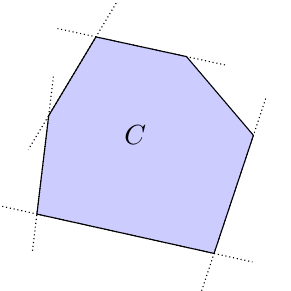
\begin{tikzpicture}[
  extended line/.style={shorten >=-#1,shorten <=-#1},,
  clip=false, scale=0.5]

    \node at (1.3, 1) (e1) {};
    \node at (-1, 1.5) (e2) {};
    \node at (3, -1) (e3) {};
    \node at (-2.2, -1/2) (e4) {};
    \node at (-2.5, -3) (e5) {};
    \node at (2, -4) (e6) {};

    \fill[blue!20] (e1.center) -- (e2.center)  -- (e4.center) -- (e5.center) -- (e6.center) -- (e3.center) -- cycle;
    \draw[black] (e1.center) -- (e2.center)  -- (e4.center) -- (e5.center) -- (e6.center) -- (e3.center) -- cycle;

    \draw[densely dotted] [extended line=0.5cm] (e1.center) -- (e2.center);
    \draw[densely dotted] [extended line=0.5cm] (e2.center) -- (e4.center);
    \draw[densely dotted] [extended line=0.5cm] (e4.center) -- (e5.center);
    \draw[densely dotted] [extended line=0.5cm] (e5.center) -- (e6.center);
    \draw[densely dotted] [extended line=0.5cm] (e6.center) -- (e3.center);
    
    \node at (0,-1) {$C$};

\end{tikzpicture}

\end{document}

%%% Local Variables:
%%% mode: latex
%%% TeX-master: t
%%% End:
